\documentclass{article}
\usepackage{setspace}
\usepackage{amsmath}
\usepackage{tikz}
\usepackage{amssymb}
\usepackage[margin=1in]{geometry}
\usepackage{xepersian}
\settextfont{Yas}
% Fixture for Xepersian 23 bug of setting persian math digit fonts
\ExplSyntaxOn\cs_set_eq:NN\etex_iffontchar:D\tex_iffontchar:D\ExplSyntaxOff
\setmathdigitfont{Yas}
\onehalfspacing
\title{
تمرین اول هوش مصنوعی
}
\author{
امیرحسین رجبی (۹۸۱۳۰۱۳)
}
\renewcommand{\labelenumi}{\alph{enumi})}
\begin{document}
	\maketitle
				\section*{
		سوال اول
	}
\begin{enumerate}
	\item 
	\item
\end{enumerate}
			\section*{
		سوال دوم
	}
	\begin{enumerate}
		\item 
		درست. بنابر توضیح کتاب در صفحه ۶۴ فصل دوم (از نسخه ۲۰۲۰) یک بازی ویدیویی جدید ممکن است صفحه بازی برای ما به طور کامل قابل مشاهده باشد ولی ندانیم که با فشردن هر دکمه چه اتفاقی خواهد افتد.
		\item 
		درست. تابع 
		\lr{transition}
		در این مدل‌ها روی فضای متناهی تعریف می‌شود و در فضاهای پیوسته پاسخگو نیست.
		\item 
		درست. اگر در الگوریتم 
		$A^*$
		تابع هیوریستیک برابر تابع ثابت صفر باشد تابع ارزیابی ($f$) همان تابع هزینه ($g$) خواهد بود.
		\item 
		نادرست. گراف زیر را در نظر بگیرید. کوتاهترین مسیر از گره $A$ به $C$ از طریق $B$ خواهد بود. اگر 
		$C = 3$
		را به تمام یال‌ها اضافه کنیم، کوتاهترین مسیر یال $AC$ خواهد بود.		
\begin{center}
			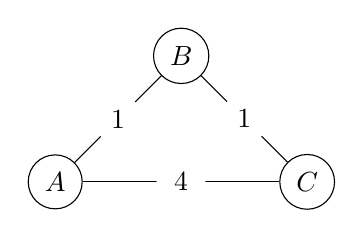
\begin{tikzpicture}[scale=0.8]
			\node[circle, draw] (A) at (0, 0) {$A$};
			\node[circle, draw] (B) at (2, 2) {$B$};
			\node[circle, draw] (C) at (4, 0) {$C$};
			\path (A) edge node[fill=white,circle] {$1$} (B);
			\path (B) edge node[fill=white,circle] {$1$} (C);
			\path (A) edge node[fill=white,circle] {$4$} (C);
		\end{tikzpicture}
\end{center}
\item
درست. می‌دانیم الگوریتم $A^*$ همه گره‌ها مانند $x$ را بسط می‌دهد که هزینه ارزیابی آنها حداکثر هزینه ارزیابی گره هدف باشد؛ یعنی اگر $n$ گره هدف باشد، 
$f(x) \leq f(n) = g(n)$. 
اما چون
$g(x) \leq g(x) + h(x) = f(x)$
پس 
$g(x) \leq g(n)$. 
بنابر شرایط گفته شده 
$g(n)$
بهینه است و در نتیجه گره $x$ توسط الگوریتم 
\lr{Uniform Cost Search}
نیز بسط داده می‌شود چرا که این الگوریتم همه گره‌ها با هزینه کمتر از 
$g(n)$
را بسط می‌دهد.
		\item 
		نادرست. مشکل اصلی 
		$A^*$
		پیچیدگی زمانی آن نیست بلکه پیچیدگی فصای مصرفی آن زیاد است. (همان طور که الگوریتم 
		$IDS$
		برای کاهش فضای مصرفی الگوریتم $BFS$ و 
		\lr{completeness}
		الگوریتم $DFS$ ارائه شد.)
			
	\end{enumerate}
		\section*{
		سوال سوم
	}
با توجه به شماره دانشجویی مسئله چهارم را حل می‌کنم. درستی گزاره را ثابت می‌کنیم. فرض کنیم گره $v$ مجاور گره $u$ باشد و هزینه انتقال از $u$ به $v$ برابر $c$ باشد. چون $x$ و $y$ تابع‌هایی 
\lr{consistent}
هستند، خواهیم داشت:
\begin{align*}
	&x(u) \leq c + x(v) \\
	&y(u) \leq c + y(v)
\end{align*}
نامساوی اول را در $\alpha$ و نامساوی دوم را در 
$1 - \alpha$
ضرب می‌کنیم: (دقت کنید به دلیل برقراری شرط $0 < \alpha < 1$ می‌توانیم بدون تغییر جهت نامساوی این کار را انجام دهیم.)
\begin{align*}
	\alpha x(u) &\leq \alpha c + \alpha x(v) \\
	(1- \alpha)y(u) &\leq (1- \alpha) c + (1- \alpha) y(v)
\end{align*}
با جمع روابط بالا داریم:
$$\alpha x(u) + (1- \alpha)y(u) \leq c + \alpha x(v) + (1- \alpha) y(v)$$
که حکم نتیجه می‌شود.
	\section*{
		سوال چهارم
	}
	مسئله اول را حل می‌‌کنیم.
	\begin{enumerate}
		\item 
		هر حالت قرارگیری $n$ پکمن در $m$ خانه نقشه یک حالت یا 
		\lr{state}
		خواهد بود. همچنین بین هر دو حالت 
		\lr{reachable}
		یک 
		\lr{transition}
		وجود دارد.
		\item 
		با توجه به بخش قبل و فرض مسئله که امکان قرارگیری چندین پکمن در یک خانه از نقشه وجود دارد، می‌توان گفت اندازه فضای حالت برابر 
		$m^n$
		خواهد بود چرا که هر پکمن می‌تواند در یکی از $m$ خانه نقشه قرار گیرد.
		\item 
		در صورتی که موقعیت همه پکمن‌ها به گونه‌ای باشد که بتوانند در هر چهار جهت بالا، پایین، چپ و راست حرکت کنند و همچنین بتوانند در جای خود باقی بمانند، تعداد یال‌های خروجی هر حالت برابر 
		$b \leq 5^n - 1$
		خواهد بود. (دقت کنید حداقل یک پکمن باید حرکت کند. در غیر این صورت درجا می‌زنیم. یک واحد به این دلیل کسر شده است.) به وضوح در صورت قرارگیری پکمن‌ها در حاشیه و مرز نقشه تعداد یال‌های خروجی آن حالت یا 
		\lr{branching factor}
		از $b$ کمتر خواهد بود. همچنین کران پایین 
		$2^n - 1 \leq b$
		را نیز داریم چرا که هر پکمن یا یک خانه مجاور دارد یا می‌تواند در جای خود باقی بماند.
		\item 
		در این مسئله تابع هزینه گام‌های مسئله 
	\LTRfootnote{Step cost function}
		عددی صحیح بین 1 و $n$ است چرا که حداقل یک پکمن یک گام حرکت کرده و همچنین حداکثر همه پکمن‌ها هر کدام یک گام حرکت می‌کنند. می‌دانیم در الگوریتم
		\lr{Uniform Cost Search}
حداکثر همه گره‌هایی بسط داده می‌شوند که مسیر بهینه آنها هزینه‌ای کمتر از پاسخ بهینه مسئله ($ C^* $) را دارد. چون تابع هزینه حداقل $\epsilon = 1$ است پس حداکثر همه گره‌ها تا عمق 
$d = \lfloor\frac{C^*}{\epsilon}\rfloor + 1 = C^* + 1$
\footnote{
دلیل وجود یک در این عبارت این است که الگوریتم 
\lr{UCS}
زمانی خاتمه می‌یابد که گره هدف را از صف اولویت خارج کند و قبل از بسط آن، هدف بودن آن را بررسی می‌کند و نه زمانی که آن را ایجاد می‌کند.
}
بسط داده می‌شوند؛ یعنی حداکثر
$b + b^2 + \cdots + b^d = \frac{b(b^{d} - 1)}{b - 1}$
گره. با توجه به بخش قبل $b$ کران پایین بزرگی دارد و می‌توانیم فرض کنیم عبارت بالا از 
$b^d$
کمتر است. از طرفی در این مسئله هر گره هدف حداکثر در عمق 
$m - 1$
خواهد بود زیرا محدودیتی برای تعداد پکمن‌هایی که می‌توانند همزمان در یک خانه از نقشه قرار داشته باشند نداریم و هر پکمن با پیمایش این تعداد گام همه‌ی خانه‌های نقشه را یک بار مشاهده می‌کند. همچنین تابع هزینه هر گام حداکثر $n$ خواهد بود. پس 
$C^* \leq n (m-1)$.
به کمک بخش قبل داریم 
$b^d \leq (5^n - 1)^{n (m-1) + 1}$.
		
	\item
	این تابع هر دو شرایط را دارد. ابتدا ثابت می‌‌کنیم تابع 
	\lr{admissible}
	است؛ یعنی تابع هیوریستیک، از هزینه واقعی بیشتر نیست. اگر مستطیل
	$R = [X_1, X_2] \times [Y_1, Y_2]$
	مستطیلی با کمترین مساحت باشد که همه پکمن‌ها درون یا روی آن قرار بگیرند، (چپ‌ترین پکمن روی خط $ x = X_1 $، راست‌ترین پکمن روی خط $ x = X_2 $، پایین‌ترین پکمن روی خط $ y = Y_1 $ و بالاترین پکمن روی خط $ y = Y_2 $ قرار می‌گیرند.) تابع هیوریستیک برابر 
	$h = \frac{1}{2}\max(X_2 - X_1, Y_2 - Y_1)$
	خواهد بود. بدون کاسته شدن از کلیت مسئله اگر 
	$h = \frac{1}{2}(X_2 - X_1)$
	و همچنین جواب بهینه برای این مسئله، ملاقات پکمن‌ها در نقطه 
	$(\alpha, \beta)$
	باشد، در این صورت اگر $\alpha \leq \frac{X_1 + X_2}{2}$، فاصله منهتن 
	\LTRfootnote{Manhattan distance}
	پکمن روی خط 
	$x = X_2$
	حداقل $h$ خواهد بود و اگر $\alpha \geq \frac{X_1 + X_2}{2}$، فاصله منهتن پکمن روی خط 
	$x = X_1$
	حداقل $h$ خواهد بود. به طوری مشابه برای 
	$h = \frac{1}{2}(Y_2 - Y_1)$
	نیز ثابت می‌شود ک $h$ کران پایینی برای هزینه واقعی حل مسئله خواهد بود.
	
	اکنون ثابت می‌کنیم تابع هیوریستیک 
	\lr{consistent}
	است. اگر $v$ گره‌ی مجاور گره‌ی $u$ باشد و هزینه انتقال از $u$ به $v$ برابر $c$ باشد، نشان می‌دهیم 
	$h(u) \leq h(v) + c$.
مستطیل‌های $ R_u $ و $ R_v $ را مانند اثبات قبل به ترتیب برای وضعیت‌های $u$ و $v$ تعریف می‌کنیم. (مستطیل‌هایی با کمترین مساحت و اضلاع موازی محور‌های مختصات که پکمن‌ها درون یا روی آنها قرار دارند.) همچنین اندازه طول مستطیل $R$ را با $L(R)$ و اندازه عرض آن را با $W(R)$ نشان می‌دهیم. بدون کاسته شدن از کلیت مسئله فرض کنیم 
	$L(R_u) \geq W(R_u)$
و در نتیجه 
$h(u) = \frac{L(R_u)}{2}$.
چون طول گام پکمن‌ها یک واحد است،
$|L(R_u) - L(R_v)| \leq 2$
و
$|W(R_u) - W(R_v)| \leq 2$
چرا که پکمن‌های روی طول یا عرض $R_u$ می‌توانند به سمت یکدیگر یا خلاف همدیگر حرکت کنند. در نتیجه 
$|h(u) - h(v)| \leq 1$.
 اگر $h(u) - h(v) = 1$، چون $ c \geq 1 $ آنگاه 
 $h(u) \leq h(v) + c$. 
 در غیر این صورت (مثلا $h(v) \geq h(u)$) رابطه
  $h(u) < h(v) + c$
   برقرار خواهد بود. پس در هر صورت داریم 
   $h(u) \leq h(v) + c$.

	\end{enumerate}
					\section*{
			گزارش پروژه
		}
	
\end{document}